

\tikzset{every picture/.style={line width=0.75pt}} %set default line width to 0.75pt        

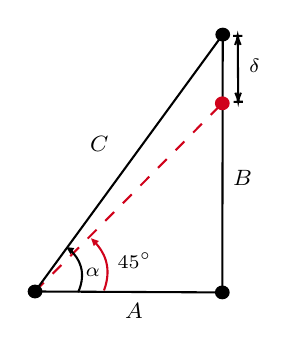
\begin{tikzpicture}[x=0.75pt,y=0.75pt,yscale=-1,xscale=1]
%uncomment if require: \path (0,300); %set diagram left start at 0, and has height of 300

%Straight Lines [id:da20080091364174113] 
\draw [color={rgb, 255:red, 208; green, 2; blue, 27 }  ,draw opacity=1 ] [dash pattern={on 4.5pt off 4.5pt}]  (59.94,139.84) -- (150.16,49.17) ;
%Straight Lines [id:da7666578220448256] 
\draw    (150.16,140.29) -- (150.27,79.78) -- (150.38,16.06) ;
%Flowchart: Connector [id:dp25706287258768046] 
\draw  [fill={rgb, 255:red, 0; green, 0; blue, 0 }  ,fill opacity=1 ] (56.89,139.84) .. controls (56.89,138.28) and (58.25,137.02) .. (59.94,137.02) .. controls (61.62,137.02) and (62.99,138.28) .. (62.99,139.84) .. controls (62.99,141.4) and (61.62,142.67) .. (59.94,142.67) .. controls (58.25,142.67) and (56.89,141.4) .. (56.89,139.84) -- cycle ;
%Flowchart: Connector [id:dp7129901164482209] 
\draw  [fill={rgb, 255:red, 0; green, 0; blue, 0 }  ,fill opacity=1 ] (147.11,140.29) .. controls (147.11,138.73) and (148.48,137.46) .. (150.16,137.46) .. controls (151.85,137.46) and (153.21,138.73) .. (153.21,140.29) .. controls (153.21,141.85) and (151.85,143.11) .. (150.16,143.11) .. controls (148.48,143.11) and (147.11,141.85) .. (147.11,140.29) -- cycle ;
%Flowchart: Connector [id:dp14605193492059754] 
\draw  [color={rgb, 255:red, 208; green, 2; blue, 27 }  ,draw opacity=1 ][fill={rgb, 255:red, 208; green, 2; blue, 27 }  ,fill opacity=1 ] (147.11,49.17) .. controls (147.11,47.61) and (148.48,46.35) .. (150.16,46.35) .. controls (151.85,46.35) and (153.21,47.61) .. (153.21,49.17) .. controls (153.21,50.74) and (151.85,52) .. (150.16,52) .. controls (148.48,52) and (147.11,50.74) .. (147.11,49.17) -- cycle ;
%Flowchart: Connector [id:dp3770909275464782] 
\draw  [fill={rgb, 255:red, 0; green, 0; blue, 0 }  ,fill opacity=1 ] (147.33,16.06) .. controls (147.33,14.5) and (148.7,13.24) .. (150.38,13.24) .. controls (152.07,13.24) and (153.43,14.5) .. (153.43,16.06) .. controls (153.43,17.62) and (152.07,18.89) .. (150.38,18.89) .. controls (148.7,18.89) and (147.33,17.62) .. (147.33,16.06) -- cycle ;
%Straight Lines [id:da4689098365411484] 
\draw    (59.94,139.84) -- (150.16,140.29) ;
%Straight Lines [id:da7092156895773364] 
\draw    (59.94,139.84) -- (150.38,16.06) ;
%Curve Lines [id:da4859163134212995] 
\draw [color={rgb, 255:red, 208; green, 2; blue, 27 }  ,draw opacity=1 ]   (93.16,139.33) .. controls (97.5,127.56) and (92.55,120.22) .. (89,116.34) ;
\draw [shift={(86.93,114.22)}, rotate = 45] [fill={rgb, 255:red, 208; green, 2; blue, 27 }  ,fill opacity=1 ][line width=0.08]  [draw opacity=0] (3.57,-1.72) -- (0,0) -- (3.57,1.72) -- cycle    ;
%Straight Lines [id:da6280238401163977] 
\draw    (157.6,16.67) -- (157.82,48.44) ;
\draw [shift={(157.82,48.44)}, rotate = 269.6] [color={rgb, 255:red, 0; green, 0; blue, 0 }  ][line width=0.75]    (0,2.24) -- (0,-2.24)(4.37,-1.32) .. controls (2.78,-0.56) and (1.32,-0.12) .. (0,0) .. controls (1.32,0.12) and (2.78,0.56) .. (4.37,1.32)   ;
\draw [shift={(157.6,16.67)}, rotate = 89.6] [color={rgb, 255:red, 0; green, 0; blue, 0 }  ][line width=0.75]    (0,2.24) -- (0,-2.24)(4.37,-1.32) .. controls (2.78,-0.56) and (1.32,-0.12) .. (0,0) .. controls (1.32,0.12) and (2.78,0.56) .. (4.37,1.32)   ;
%Curve Lines [id:da9497681171147138] 
\draw [color={rgb, 255:red, 0; green, 0; blue, 0 }  ,draw opacity=1 ]   (80.71,140.22) .. controls (85.08,130.38) and (80.94,123.68) .. (77.22,120.24) ;
\draw [shift={(74.93,118.44)}, rotate = 32.91] [fill={rgb, 255:red, 0; green, 0; blue, 0 }  ,fill opacity=1 ][line width=0.08]  [draw opacity=0] (3.57,-1.72) -- (0,0) -- (3.57,1.72) -- cycle    ;

% Text Node
\draw (90.04,130.54) node  [font=\scriptsize] [align=left] {\begin{minipage}[lt]{8.67pt}\setlength\topsep{0pt}
$\displaystyle \alpha $
\end{minipage}};
% Text Node
\draw (98.27,119.43) node [anchor=north west][inner sep=0.75pt]  [font=\scriptsize] [align=left] {$\displaystyle 45^{\circ }$};
% Text Node
\draw (84.93,63.6) node [anchor=north west][inner sep=0.75pt]  [font=\footnotesize] [align=left] {$\displaystyle C$};
% Text Node
\draw (101.82,144.04) node [anchor=north west][inner sep=0.75pt]  [font=\footnotesize] [align=left] {$\displaystyle A$};
% Text Node
\draw (153.82,80.04) node [anchor=north west][inner sep=0.75pt]  [font=\footnotesize] [align=left] {$\displaystyle B$};
% Text Node
\draw (161.6,26.49) node [anchor=north west][inner sep=0.75pt]  [font=\scriptsize] [align=left] {$\displaystyle \delta$};


\end{tikzpicture}
